\documentclass{beamer}
\usepackage{xmpmulti}
\usepackage{caption}
\usepackage{subcaption}
\usepackage{epstopdf}
\usepackage{graphics}
\usepackage{tikz}
\usepackage{amsmath}
\usepackage{verbatim}
\usepackage{color}
\definecolor{links}{HTML}{2A1B81}
\hypersetup{colorlinks,linkcolor=,urlcolor=links}
\setbeamertemplate{navigation symbols}{}

\usetheme{Darmstadt}
%\setbeameroption{show notes}
\beamersetuncovermixins{\opaqueness<1>{25}}{\opaqueness<2->{15}}

\date{\today}

\begin{document}


\title{Cognitive Ecology: A Framework for Cognitively Heterogenous Agents.}
%Here's how I can see your paper:
%A) motivation of big project: aggregation of diverse beliefs. Want to measure relationship of diverse beliefs to performance
%B) This paper: describing causal beliefs and measuring diversity
%C) In math, define a causal belief structure, and relate it to a probability density function
%D) In math, show how the Weitzman measure + the JS metric yield a measure of the diversity of probability density functions.
%E) In a simulation, describe 5 macroeconomic variables, create say 10 causal belief structures out of them.
%F) Specify the resulting probability density functions. Calculate diversity.
%G) Show that as you change how you create the 10 causal belief structures, the diversity measure changes in a plausible way.
%H)Conclude.



\author{Johannes Castner}
\institute{Columbia University}
\begin{frame}
\titlepage
\begin{center}
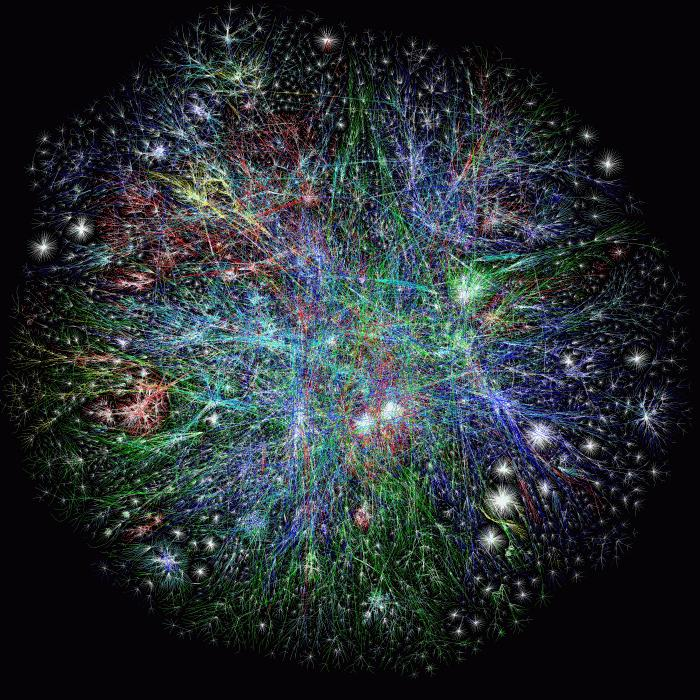
\includegraphics[scale=0.1]{complexity.jpeg}
\end{center}

\end{frame}

\frame{\frametitle{Table of contents}\tableofcontents}
\section{Motivation}
\begin{frame}
\frametitle{Motivations and Questions}
My Motivations are twofold:
\begin{itemize}
\item Short Run: theorize and show empirically that more Cognitive Diversity can be advantageous for an organization or a group.
\item Long Run: help to build a cognitive foundation for the social sciences (theoretically and empirically), wherein individuals are really individuals and not clones of each other.
\end{itemize}
\end{frame}
\begin{frame}
\frametitle{Cognitive Diversity vs. Diversity in Preferences}
Economics and Political Science, are focused on differences in
\begin{itemize}
\item goals and preferences
\item information asymmetries.
\end{itemize}
\textcolor{red}{But what if information and goals are the same, but beliefs are heterogenous?}
\begin{itemize}
\item when people work in a team
\end{itemize}
\textcolor{red}{Or what if both, beliefs and goals are heterogenous?}
\begin{itemize}
\item Is climate change policy a matter of goals or a matter of beliefs, or both?
\end{itemize}
\end{frame}
\begin{frame}
\frametitle{``Cognitive Diversity'' in teams.}
For the moment, loosely define ``Cognitive Diversity'' as a quantitative measure of \textit{within group} heterogeneity of belief systems (causal beliefs about the world).\\

The Questions are:\\
\begin{itemize}
\item Does greater ``Cognitive Diversity'' lead to better group decisions, when the goals of all members are well-matched; and how?
\item How and under what forms of Belief Aggregation is ``Cognitive Diversity'' best utilized?
\end{itemize}
\end{frame}
\begin{frame}
\frametitle{Condorcet's jury theorem}
My work builds on Marquis de Condorcet's ``Essay on the Application of Analysis to the Probability of Majority Decisions'' (1785).\\
Assumptions:
\begin{itemize}
\item group wishes to reach a decision by majority vote.
\item One of two potential outcomes of the vote is correct.
\item each voter has an independent probability, $p$, of voting for the correct decision.
\end{itemize}
How many voters should we admit to the group?\\
Answer:
\begin{itemize}
\item if $p> \frac{1}{2}$ admit as many voters as possible (in the limit the probability that the majority decision is correct is $1$)
\item if $p<\frac{1}{2}$ admit only one voter!
\end{itemize}
\end{frame}
\begin{frame}
\frametitle{Beyond the Condorcet's Jury Theorem}
Condorcet's Jury Theorem is one-dimensional and it doesn't include Diversity (i.e. the only diversity is coming from the independents of each person's probability of being right).\\
\begin{itemize}
\item For $n$ people, the probability of $k$ being correct is:
$$Pr(k)=\frac{n!}{k!(n-k)!} * p^k(1-p)^{n-k}$$
\item So we need to calculate
$$Pr(k>\frac{1}{2}*n)=\sum_{k>\frac{1}{2}*n}\frac{n!}{k!(n-k)!} * p^k(1-p)^{n-k}$$
\item But also: it is a one-shot decision with no learning.\\
\end{itemize}
What if an organization can weigh the votes after learning something about the accuracy of each belief?\\
Suppose we have a partial ranking $p_1 \geq p_i \geq \cdots\geq p_n$ over at least some of the $n$ beliefs, based on evidence?
\end{frame}
\begin{frame}
\frametitle{Model derived multi-demsional joint-probabilities}
Main departures from Condorcet's Jury Theorem:
\begin{itemize}
\item Probabilities are over vectors of variables, $v_1, \ldots, v_n$.
\item Joint-distributions come from causal mental models of the world
\item Mental models can be compared with each other
\item and evaluated against data (using Bayesian Updating)
\item Mental models can evolve over time
\item The theory is about \textit{Diversity} and not just \textit{Quantity}
\end{itemize}
In fact, if two identical models are present, the Diversity is no greater than if only one of the two are present.\\
\textcolor{red}{Thus, my work is very different from the Condorcet's Jury Theorem after all.}
\end{frame}
\section{Debt}
\begin{frame}
\frametitle{The Giants on whose shoulders I'm trying to stand}
\begin{itemize}
\item Robert Axelrod and collaborators (Structure of Decision, 1976), Cognitive Maps.

\item Cognitive Scientists Tom Griffiths (Berkeley) and Joshua Tennenbaum (MIT) for Bayesian Models of Causal Cognition.

\item Scott Page (Michigan University) has first built models to show the importance of cognitive diversity. His work inspired mine.

\end{itemize}

\end{frame}

\section{A Modular Research Program}
\begin{frame}
\frametitle{A Modular Research Program}
\begin{quotation}
We have now assigned to reason and experience their place within the system of theoretical physics. Reason gives the structure to the system; the data of experience and their mutual relations are to correspond exactly to consequences in the theory. On the possibility alone of such a correspondence rests the value and the justification of the whole system, and especially of its fundamental concepts and basic laws.
\end{quotation}
\begin{flushright}
-Albert Einstein
\end{flushright}

My overall research goals are big, but each piece is small. Each theoretical piece must have the possibility of an empirical counterpart.
\end{frame}

\section{The Pieces (Modules)}
\begin{frame}
\frametitle{The Pieces (Modules)}
My research approach is modular and here are some of the modules (the first three are foundations, layed by others):
\begin{itemize}
\item What are Mental Models and how can they be elicited from people through interviews and texts? (Axelrod et. al 1976)
\item Encoding Mental Models as Bayesian Networks (Joint Prior Distributions). (following Tennenbaum and Griffiths, 2003, 2004, 2005)
\item Parameterizing Prior Distribution (Pearl, 1988).
\item Bayesian updating and a Theory of Social Influence (A sketch).
\item Measures of Cognitive Distance and Cognitive Diversity.
\end{itemize}
\end{frame}
\section{Mental Models}
\begin{frame}
\frametitle{Mental Models (Cognitive Maps)}
Mental Models of interest here are Causal Models over some restricted domain (Axelrod et. al 1976).

For Macro-Economists, for example, the universe of interest includes variables such as
\begin{itemize}
\item Interest Rates,
\item Unemployement,
\item GDP,
\item Inflation etc.
\end{itemize}
Models could be Neo-classical and Keynesian, for example, but many more models are possible and in fact exist in the minds of policy makers (Neo-classical and Keynesian are stereotypes).
\end{frame}

\begin{frame}
\frametitle{Cognitive Maps as Directed Signed Graphs}
\begin{figure}
        \centering
        \begin{subfigure}[b]{0.3\textwidth}
                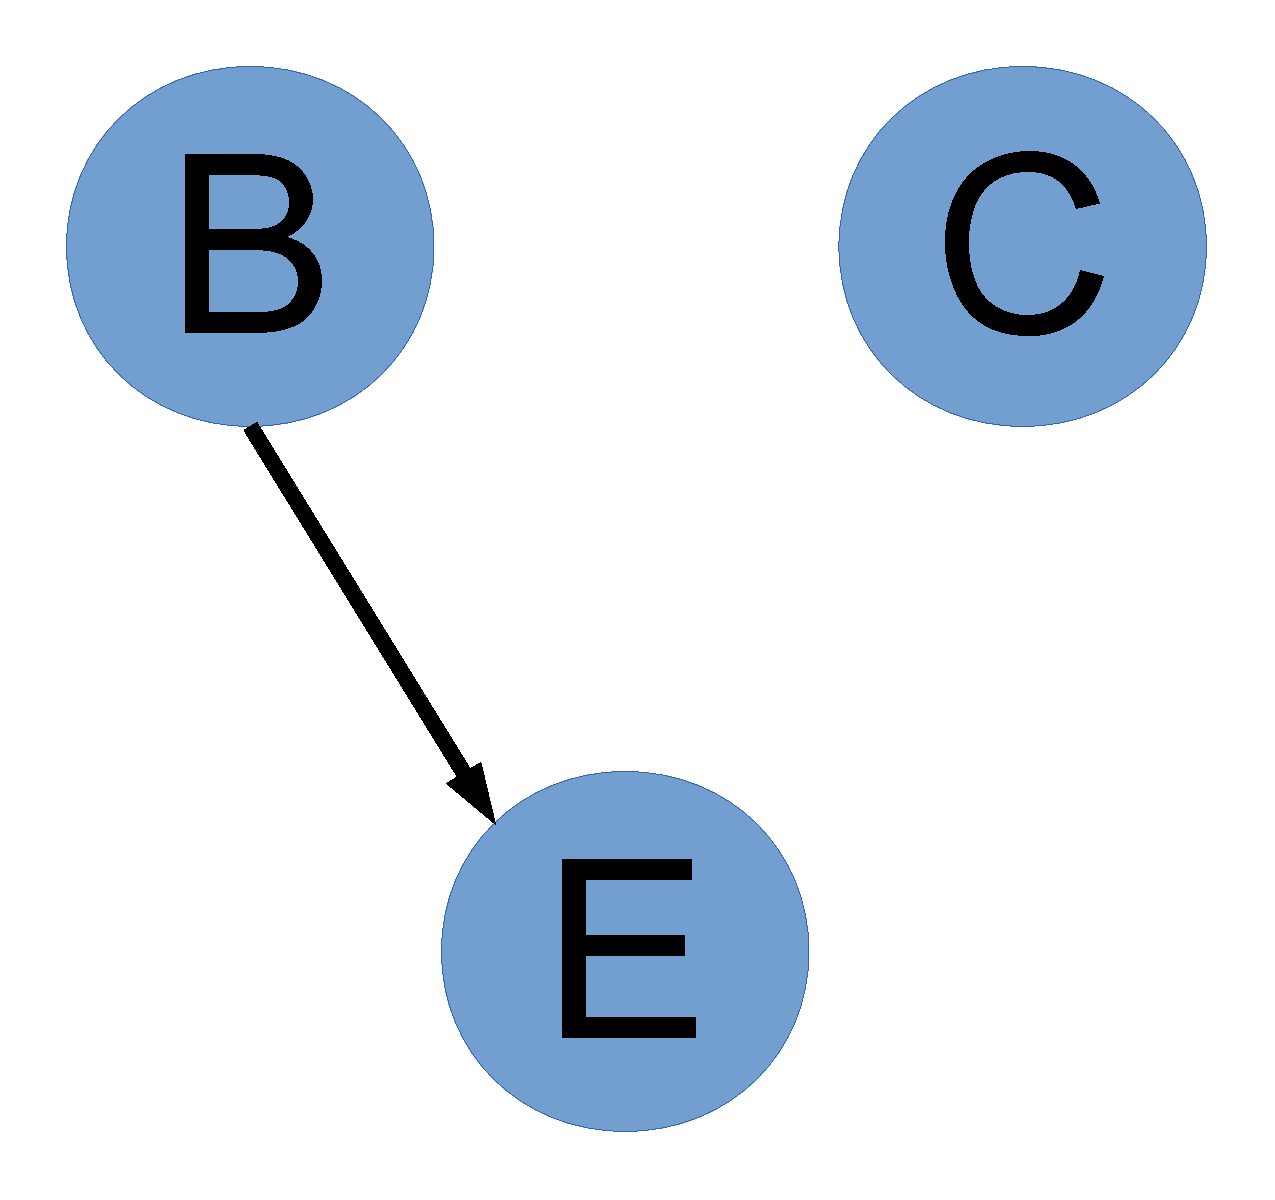
\includegraphics[width=\textwidth]{Graph0.pdf}
                \caption{Graph 0}
                \label{fig:gull}
        \end{subfigure}%
        ~ %add desired spacing between images, e. g. ~, \quad, \qquad etc.
          %(or a blank line to force the subfigure onto a new line)
        \begin{subfigure}[b]{0.3\textwidth}
                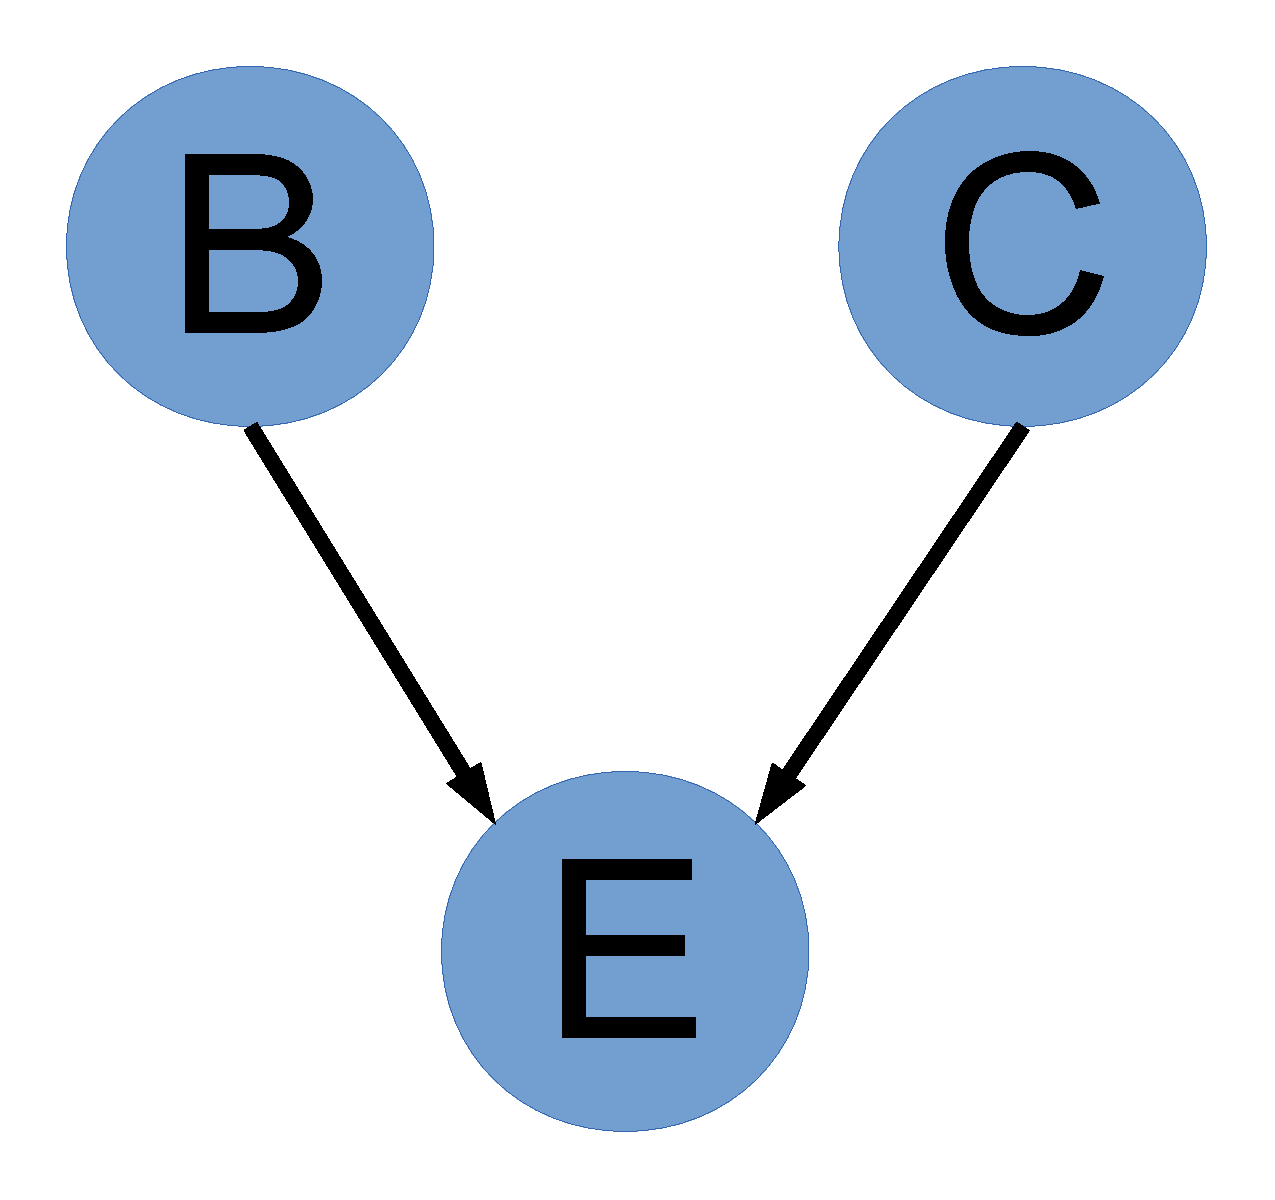
\includegraphics[width=\textwidth]{Graph1.pdf}
                \caption{Graph 1}
                \label{fig:tiger}
        \end{subfigure}
        ~ %add desired spacing between images, e. g. ~, \quad, \qquad etc.
          %(or a blank line to force the subfigure onto a new line)
        \caption{Two examples of Simple Cognitive Maps}\label{fig:animals}
\end{figure}
Here ``B'' stands for Background Cause and ``C'' stands for Cause (the causal variable believed in by actor 1, but not by actor 0).
\end{frame}

\begin{frame}
\frametitle{Non-Linearities}
There are two seeming restrictions:
\begin{itemize}
\item A relational restriction: ``$A$ has a positive/negative causal effect on $B$'',\\
\begin{center}
\textcolor{red}{The Poblem:}\\
\end{center}
 When relations are non-linear (as in the Laffer Curve).
\begin{center}
\textcolor{green}{The Solution:}\\
\end{center}
The statement ``Taxes have a negative effect on output'' has to be interpreted as: ``the instantaneous effect of taxes on output is negative, conditional on the current level of taxes and output.''\\
\end{itemize}
\end{frame}
\begin{frame}
\frametitle{Causal Loops}
\begin{itemize}
\item A structural restriction: Belief Systems can not include causal cycles\\
\begin{center}
\textcolor{red}{The Poblem:}\\
\end{center}
When someone expresses beliefs in equilibria (negative causal feedback cycles) as most economists do, or in runaway effects (positive causal cycles), as some climate scientists do.
\begin{center}
\textcolor{green}{The Solution:}\\
\end{center}
Including a time dimension (with possibly very short time-intervals).
\end{itemize}
$$A_{t=0}\rightarrow B_{t=1} \rightarrow A_{t=2}\rightarrow B_{t=3}\rightarrow \cdots$$
\end{frame}


\begin{frame}
\frametitle{Eliciting Cognitive Maps: Empirical Data on Beliefs}
How beliefs are elicited and Cognitive Maps are constructed from statements is detailed in ``Structure of Decision: The Cognitive Maps of Political Elites'' (1976), edited by Political Scientist Robert Axelrod.

Basic Idea:

\begin{itemize}
\item Either use interview or use transcriptions of speeches/debates
\item get statements of the form: CO$_2$ causes Climate Change
\item encode as directed signed arc of the graph representing a particular actor's belief system:
$$\text{CO}_2 \rightarrow^+ \text{Climate-Change}$$
\end{itemize}
\end{frame}
\section{Bayesian Beliefs}
\begin{frame}
\frametitle{Encoding Cognitive Maps as Bayesian Networks}
Why Bayesian Networks? Current and planned work:

\begin{itemize}
\item For a natural dynamic theory of belief updating and causal learning (Griffiths and Tennenbaum).
\item For a theory of social (media) influence, where belief systems are well defined objects.
\item For meaningful measures of Cognitive Distance and Cognitive Diversity.
\item For theories of Belief Aggregation and Belief Synthesis
\item For a theory of Belief System Evolution (including random mutations in the learning process to explore the belief space)
\end{itemize}
Bayesian Networks (together with Bayesian Updating, or Biased Bayesian Updating) are very useful for modeling dynamic processes involving belief systems.
\end{frame}
\begin{frame}
\frametitle{Some Foundations}
The following introduction to the Bayesian Network representation of individual Belief Systems closely follows:\\
\href{http://cocosci.berkeley.edu/tom/papers/bayeschapter.pdf}{Griffiths, T. L., Kemp, C., and Tenenbaum, J. B. (2008). ``Bayesian models of cognition.'' In Ron Sun (ed.), The Cambridge handbook of computational cognitive modeling. Cambridge University Press.}

\end{frame}
\begin{frame}
\frametitle{Encoding Cognitive Maps as Bayesian Networks}
The problem of learning the ``correct'' causal graphical model has two aspects:
\begin{itemize}
\item Model Selection,
and
\item Parameter Estimation.
\end{itemize}
Where, if we have someone's Cognitive Map at a given time, we have his ``class of models,'' that is, we know the class of models that the actor has \textit{selected} (based on previous deliberation and experience) up to the particular ``parameterization'', which we do \textit{not} know.
\end{frame}

\begin{frame}
\frametitle{Encoding Cognitive Maps as Bayesian Networks}
\begin{figure}

  \centering
    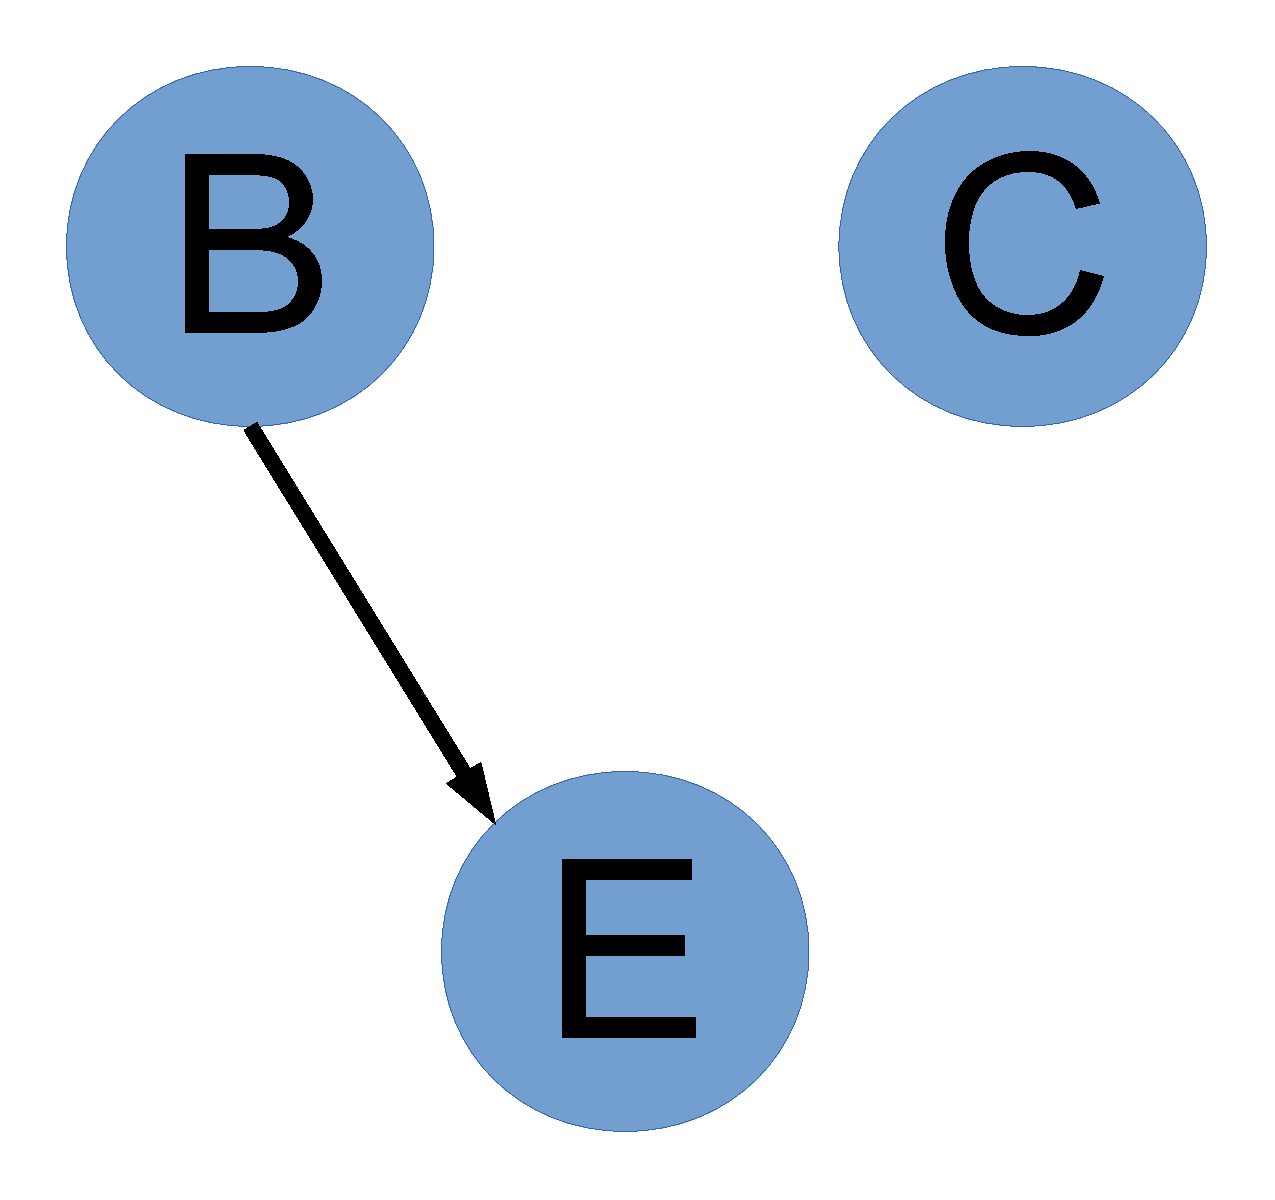
\includegraphics[width=0.2\textwidth]{Graph0.pdf}
\end{figure}

Graph$_0$ is encoded as follows as a Bayesian Network (or simply joint distribution). The joint distribution of any $k$ variables ($k=3$ in this case) can be written as the product of all of its conditionals and its marginals. In the case of Graph$_0$:
$$P_0(B, C, E)= P(E | B)*P(B)*P(C)$$

Note that since $B$ is believed to cause $E$, the value of $E$ is believed to depend on the value of $B$ and thus the term $P(E | B)$ is included. However, $E$ is independent from $C$ and thus $P(E | B, C)$ collapses, while in Graph$_1$ the term would have to be $P(E | B, C)$.
\end{frame}

\begin{frame}
\frametitle{Encoding a Causal Arc}
\begin{figure}

  \centering
    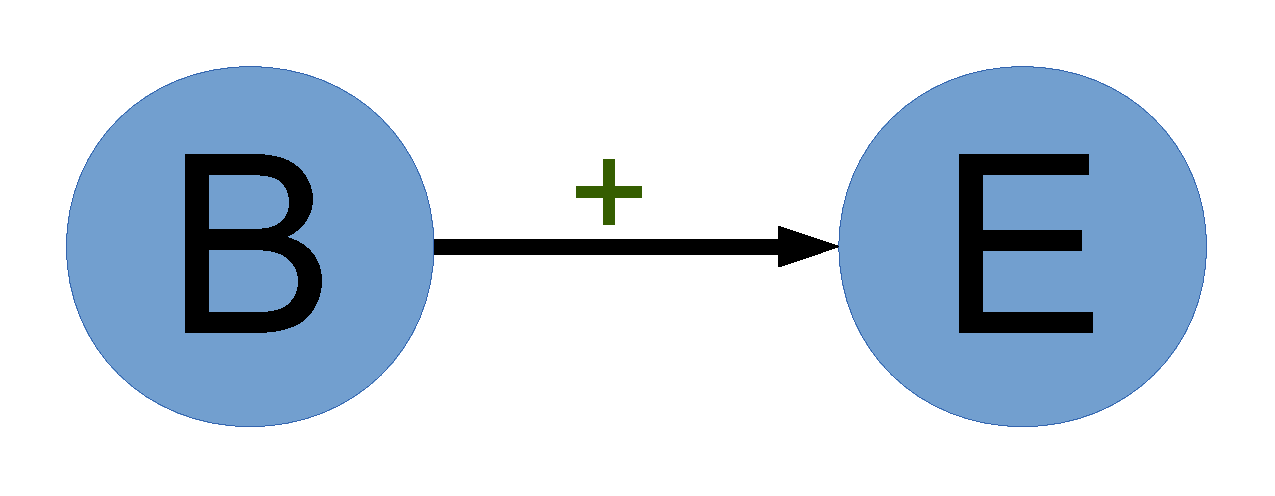
\includegraphics[width=0.5\textwidth]{Cause+.pdf}
\end{figure}
For a positive causal relation, where B is the cause of E, we have
$$P(E=1 | B=1) > P(E=1 | B=0)$$
for binary random variables B and E. For this discussion, I assume that all variables are binary, but similar encoding can be done for numerical variables of all sorts (discrete or continuous).
\end{frame}
 \begin{frame}
\frametitle{Contingency Tables}

Contingency Table Representation used in Elemental Causal Induction:
\begin{center}
    \begin{tabular}{l l l}
    & Effect Present ($e^+$) & Effect Absent ($e^-$) \\\hline
    Cause Present ($c^+$) & N($e^+$, $c^+$) & N($e^-$, $c^+$)  \\
    Cause Absent ($c^-$) & N($e^+$, $c^-$) & N($e^-$, $c^-$)  \\
    \hline
    \end{tabular}
\end{center}
 Jenkins and Ward (1965) suggest that the degree of causation is best measured by the quantity (estimated from data using contingency counts, N($\cdot$)):
$$\Delta P = \frac{\text{N($e^+$, $c^+$)}}{\text{N($e^+$, $c^+$)}+\text{N($e^-$, $c^+$)}}-\frac{\text{N($e^+$, $c^-$)}}{\text{N($e^+$, $c^-$)}+\text{N($e^-$, $c^-$)}}=$$
$$P(e^+, c^+)-P(e^+, c^-)$$
\end{frame}

 \begin{frame}
\frametitle{$\Delta P$ and Causal Power (Updating Rules)}
Remember (previous slide) that
$$\Delta P= P(e^+, c^+)-P(e^+, c^-)$$
Cheng (1997) suggested that people’s judgments are better captured by ``causal power'':

$$Power=\frac{\Delta P}{1-P(e^+ | c^-)},$$
which predicts that $\Delta P$ will have a greater effect when $P(e^+ | c^-)$ is large.

\end{frame}

\begin{frame}
\frametitle{Parameterization of Beliefs, the trivial case}
We need to define the form of the conditional probability distribution, $P(E | B, C)$, which is called the ``parameterization of the Graph.'' \\

For Graph$_0$ this can simply be done with one parameter: $P_0(E=e^+ | B=b, \omega_{0, 0})=\omega_{0, 0}b$, where $b \in \{0, 1\}$.

$$\Delta_b P_0= P_0(e^+, b^+)-P_0(e^+, b^-) = \omega_{0, 0}$$
\end{frame}

\begin{frame}
\frametitle{Parameterization of Beliefs, the less trivial case}

For Graph$_1$ we could also write
$$\Delta_b P_1= P_1(e^+, b^+)-P_1(e^+, b^-) = \omega_{1, 0}$$
and
$$\Delta_c P_1= P_1(e^+, c^+)-P_1(e^+, c^-) = \omega_{1, 1}.$$
But can we write:
$$P(E | B, C)= \omega_{1, 0}*B + \omega_{1, 1}*C,$$
as in a simple, linear regression?
\end{frame}

\begin{frame}
\frametitle{Parameterization of Beliefs, the less trivial case}
Can we write $P(E | B, C)= \omega_{1, 0}*B + \omega_{1, 1}*C?$\\
We know that $0<P(E | B, C) < 1$, because it is a probability. But then,
$$0<\omega_{1, 0} + \omega_{1, 1} <1,$$
which is a dependence between the parameters $\omega_{1, 0}$, $\omega_{1, 1}$ that didn't come explicitly out of the beliefs.
\end{frame}

\begin{frame}
\frametitle{The ``Noisy-OR'' Parameterization (Pearl, 1988)}
\begin{figure}

 \centering
    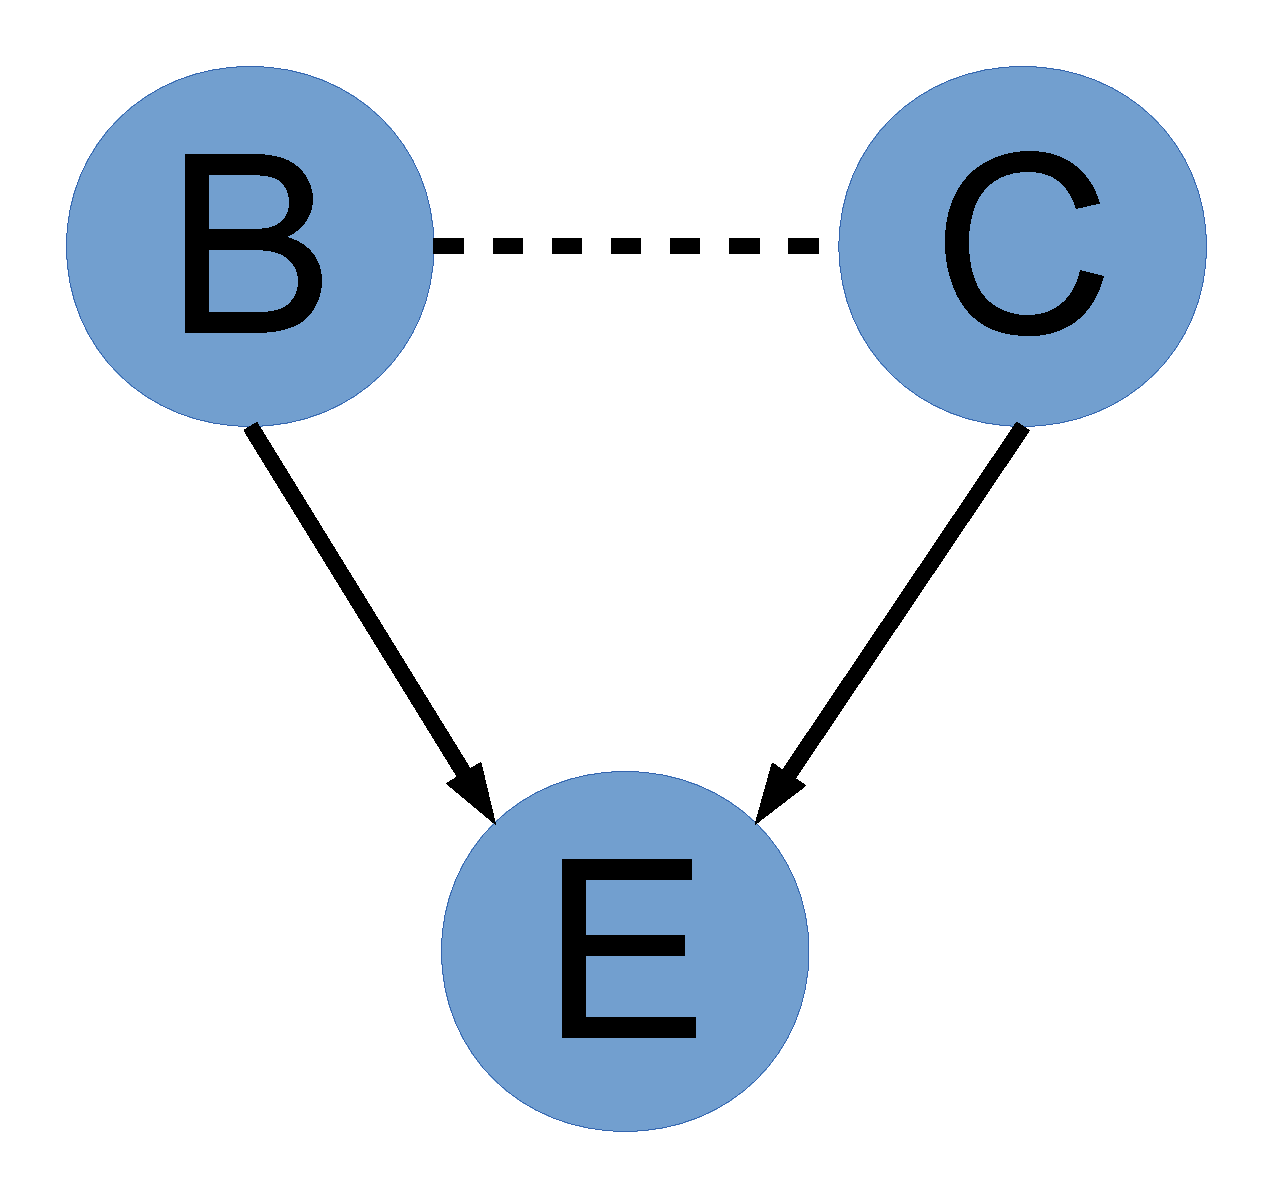
\includegraphics[width=0.2\textwidth]{GraphDep.pdf}
\end{figure}
To break this artificial dependency, the ``Noisy-OR'' parameterization (Pearl, 1988) is used:

$$P_1(e^+ | b, c, \omega_{1, 0}, \omega_{1, 1})=1-(1-\omega_{1, 0})^b *(1-\omega_{1, 1})^c$$

which breaks the dependency between $\omega_{1, 0}$ and $\omega_{1, 1}$.
\end{frame}

\begin{frame}
\frametitle{The ``Noisy-OR'' Parameterization}
$$P_1(e^+ | b, c, \omega_{1, 0}, \omega_{1, 1})=1-(1-\omega_{1, 0})^b *(1-\omega_{1, 1})^c,$$
gives that
$$P_1(e^+ | B=1, C=0, \omega_{1, 0}, \omega_{1, 1})=\omega_{1, 0},$$
$$P_1(e^+ | B=0, C=1, \omega_{1, 0}, \omega_{1, 1})=\omega_{1, 1}$$
and
$$P_1(e^+ | B=1, C=1, \omega_{1, 0}, \omega_{1, 1})=\omega_{1, 0} + \omega_{1, 1} -\omega_{1, 0}*\omega_{1, 1}.$$
If $\omega_{1, 0}=\omega_{1, 1}=1$, the ``Noisy-OR'' becomes the \textit{or}-function:\\
$E=1$ whenever $B=1$, or $C=1$ or both, $E=0$ otherwise.
\end{frame}

\begin{frame}
\frametitle{Psychology and parameterizing beliefs}
Two important theories as to how people update their causal beliefs:
\begin{itemize}
\item $\Delta P = P(e^+ | c^+)-P(e^+ | c^-)$
\item Causal Power ($\frac{\Delta P}{1-P(e^+ | c^-)}$).
\end{itemize}
Tenenbaum and Griffiths (2001, 2005) showed that both psychological theories correspond to maximum-likelihood estimates of the causal strength parameter $\omega_{1, 1}$:
\begin{itemize}
\item $\Delta P$ results from assuming the linear parameterization
\item and Causal Power results from the ``Noisy-OR'' parameterization.
\end{itemize}
As the ``Noisy-OR'' parameterization is logically more sound, I will use a Causal Power Likelihood, along with a ``Noisy-OR'' parameterization.
\end{frame}
\section{Cognition and Social Science}
\begin{frame}
\frametitle{Two Cognitive Maps as two Hypotheses}
\begin{figure}
        \centering
        \begin{subfigure}[b]{0.2\textwidth}
                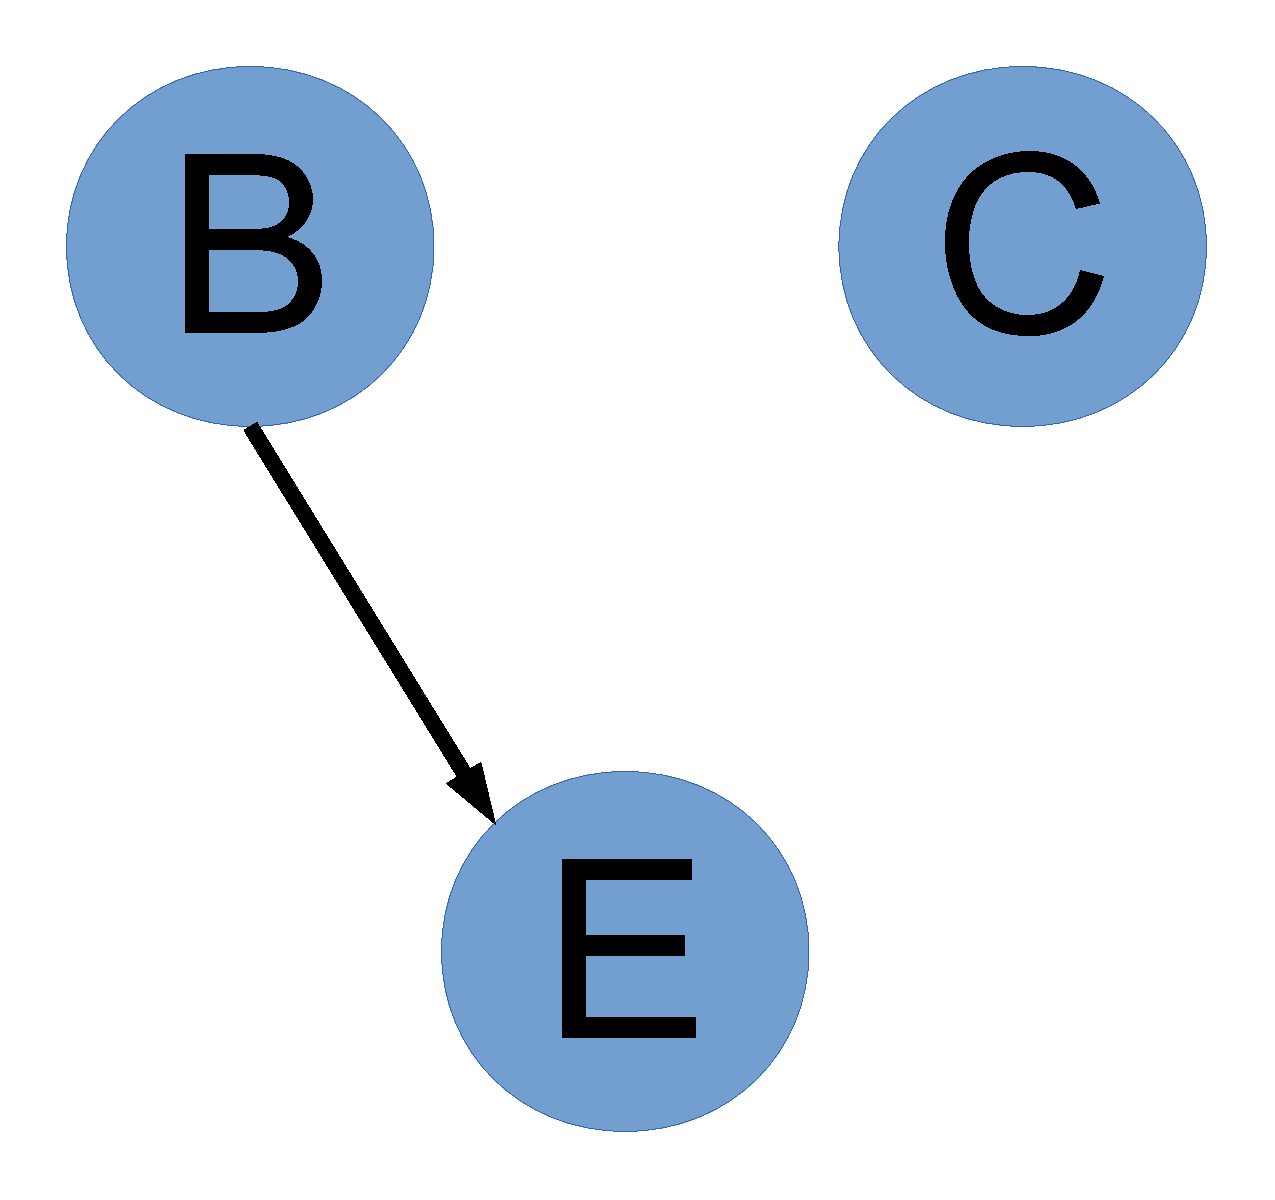
\includegraphics[width=\textwidth]{Graph0.pdf}
                \caption{Graph 0}
                \label{fig:gull}
        \end{subfigure}%
        ~ %add desired spacing between images, e. g. ~, \quad, \qquad etc.
          %(or a blank line to force the subfigure onto a new line)
        \begin{subfigure}[b]{0.2\textwidth}
                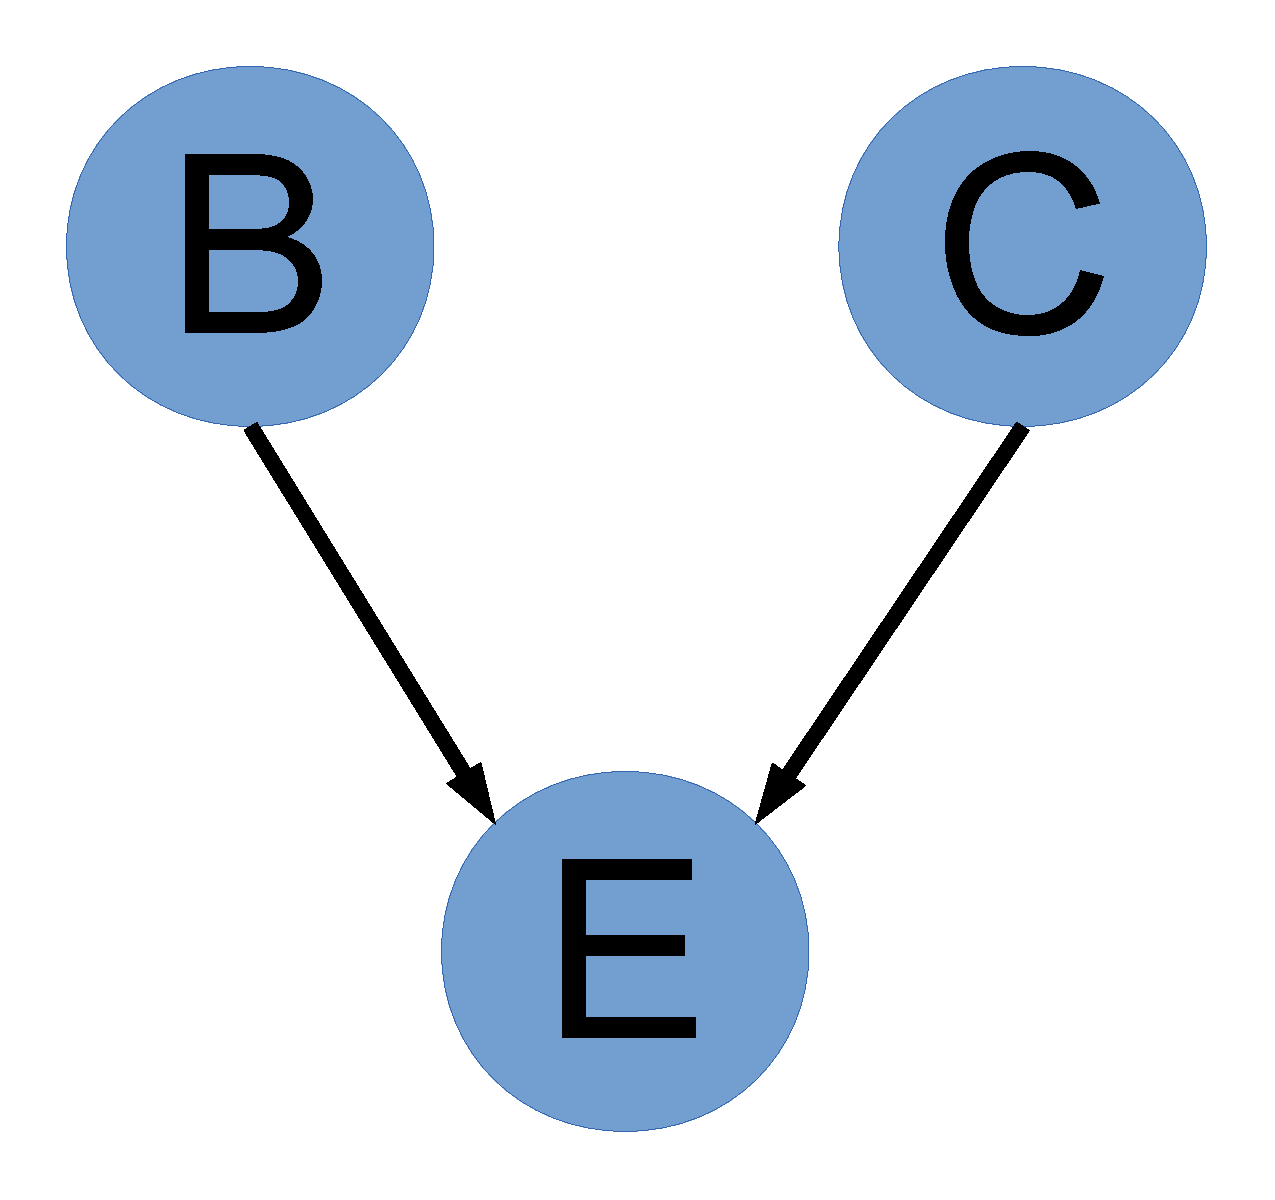
\includegraphics[width=\textwidth]{Graph1.pdf}
                \caption{Graph 1}
                \label{fig:tiger}
        \end{subfigure}
        ~ %add desired spacing between images, e. g. ~, \quad, \qquad etc.
          %(or a blank line to force the subfigure onto a new line)
\end{figure}
If we have some data of the world, $D$, we can write the \textit{posterior odds} as follows:
$$\frac{P(\text{Graph}_1 | D)}{P(\text{Graph}_0 | D)} = \frac{P(D | \text{Graph}_1)}{P(D | \text{Graph}_0)} \frac{P(\text{Graph}_1)}{P(\text{Graph}_0)}$$
\end{frame}

\begin{frame}
\frametitle{Likelihood ratio and Prior Odds Ratio}
$$\overbrace{\frac{P(\text{Graph}_1 | D)}{P(\text{Graph}_0 | D)}}^\text{\textcolor{blue}{Posterior Odds}} = \overbrace{\frac{P(D | \text{Graph}_1)}{P(D | \text{Graph}_0)}}^\text{\textcolor{green}{Likelihood Ratio}} \overbrace{\frac{P(\text{Graph}_1)}{P(\text{Graph}_0)}}^\text{\textcolor{red}{Prior Odds}}$$
\textcolor{green}{The Likelihood Ratio:}
$$\frac{P(D | \text{Graph}_1)}{P(D | \text{Graph}_0)}=$$
$$\frac{P_1(E=e | B=b, C=c)*P_1(B=b)*P_1(C=c)}{P_0(E=e | B=b)*P_0(B=b)*P_0(C=c)},$$
where I use the ``Noisy-OR'' parameterization of $P_1$, $P_0$ (Pearl, 1988).
\end{frame}
\begin{frame}
\frametitle{The Likelihood Function (updating)}
The question that the Likelihood Function answers is the following:
\begin{center}
Given our model of the world, how plausible is the data that we are experiencing?
\end{center}
For example:
$$P_1(B=1, C=1, E=1) =\pi_{1,b}, * \pi_{1,c} * \left(\omega_{1, 0} + \omega_{1, 1} - \omega_{1, 0} * \omega_{1, 1}\right),$$
where $\pi_{1,b}$ and $\pi_{1,c}$ are the parameters associated with the marginal probabilities of our ``un-caused'' variables, $P_1(B=1)$ and $P_1(C=1)$.
\end{frame}
\begin{frame}
\frametitle{The Likelihood Ratio}
\textcolor{green}{The Likelihood Ratio:}\\
suppose $D=(B=1, C=1, E=1)$ then the \textcolor{green}{Likelihood Ratio} is:
$$\frac{P_1(B=1, C=1, E=1)}{P_0(B=1, C=1, E=1)} = \frac{\pi_{1,b}, * \pi_{1,c} * \left(\omega_{1, 0} + \omega_{1, 1} - \omega_{1, 0} * \omega_{1, 1}\right)}{\pi_{0,b}, * \pi_{0,c} * \omega_{0, 0}}.$$
But note that $P_1(B=0, C=1, E=1)=\pi_{1, c} *\omega_{1, 1}>0$, while $P_0(B=0, C=1, E=1)=\pi_{0, c}* 0 = 0$, so that the Likelihood Ratio is undefined when $D=(B=0, C=1, E=1)$!\\
In that case, we just say that the ratio is infinite and Model$_1$, explains that data infinitely better than Model$_0$, no matter what the prior was.
\end{frame}
\begin{frame}
\frametitle{The Prior and Posterior Odds as Basis for a Theory of Trust and Social Influence}
Suppose that you have two friends, call them $1$, and $0$, endowed with beliefs specified by Graph$_1$ and Graph$_0$ respectively.

If you trust $1$'s opinion more than $0$s opinion, then $P(\text{Graph}_1)>P(\text{Graph}_0)$ and the prior odds ratio of the two graphs is greater than $1$. Otherwise, if you trust $0$ more than $1$, the prior odds ratio of their two models (if $1$ is in the numerator) is a positive fraction.
\end{frame}

\begin{frame}
\frametitle{Persuasion Processes}
The above suggests how the modeling of belief updating (learning) can be made to include social influence in a straight forward and natural way.

Updating uses data to evaluate ones own and others opinions, particularly those peoples' opinions with whom the actor has contact.

And of course, media influence can be studied using this framework!

$$\overbrace{\frac{P(\text{Graph}_1 | D)}{P(\text{Graph}_0 | D)}}^\text{\textcolor{blue}{Relative Trust$_{1, 0, t=1}$}} = \overbrace{\frac{P(D | \text{Graph}_1)}{P(D | \text{Graph}_0)}}^\text{\textcolor{green}{New Evidence$_{1, 0}$}} \overbrace{\frac{P(\text{Graph}_1)}{P(\text{Graph}_0)}}^\text{\textcolor{red}{Relative Trust$_{1, 0, t=0}$}}$$
By comparing ones own model and ones friends' models, in light of data, one might be swayed over time to find a more likely synthesis. This swaying process is made precise with Bayesian model comparison, where initial biases are expressed as prior odds.
\end{frame}
\begin{frame}
\frametitle{Biases and Evidence}
Again, we have:
$$\overbrace{\frac{P(\text{Graph}_1 | D)}{P(\text{Graph}_0 | D)}}^\text{\textcolor{blue}{Posterior Odds}} = \overbrace{\frac{P(D | \text{Graph}_1)}{P(D | \text{Graph}_0)}}^\text{\textcolor{green}{Likelihood Ratio}} \overbrace{\frac{P(\text{Graph}_1)}{P(\text{Graph}_0)}}^\text{\textcolor{red}{Prior Odds}}.$$
Taking the $\log$ gives:
$$\overbrace{\log\left(\frac{P(\text{Graph}_1 | D)}{P(\text{Graph}_0 | D)}\right)}^\text{\textcolor{blue}{Log Posterior Odds}} = \overbrace{\log\left(\frac{P(D | \text{Graph}_1)}{P(D | \text{Graph}_0)}\right)}^\text{\textcolor{green}{Log Likelihood Ratio}} + \overbrace{\log\left(\frac{P(\text{Graph}_1)}{P(\text{Graph}_0)}\right)}^\text{\textcolor{red}{Log Prior Odds}}.$$
While the Posterior Ratio ranges from $0$ to $\infty$, the Log Posterior Ratio ranges from $-\infty$ to $\infty$ and is $0$ when both models are believed to be equally plausible (or equally implausible).
\end{frame}
\begin{frame}
\frametitle{Causal Support}
We say that Model$_1$ is better supported by $D$ then Model$_0$ whenever:
$$\log\left(\frac{P(D | \text{Graph}_1)}{P(D | \text{Graph}_0)}\right) >0$$
and this is why, in the context of Causal Models, Tenenbaum and Griffiths renamed the Log Likelihood Ratio the \textcolor{green}{``Causal Support''} of Model$_1$ against Model$_0$.\\
The \textcolor{red}{magnitude} of the \textcolor{red}{difference in explanatory power} matters and is meaningful.
\end{frame}
\begin{frame}
\frametitle{Calculating ``Causal Support''}
We have that the ``Causal Support'' is
$$\text{Causal Support} = \log\left(\frac{P(D | \text{Graph}_1)}{P(D | \text{Graph}_0)}\right).$$
Not wanting to introduce artificial differences (that we don't know from data), we assume:
$$\pi_{1, b} =\pi_{0, b} \text{ and } \pi_{1, c} =\pi_{0, c},$$
so that these parameters cancel out.
\end{frame}
\begin{frame}
\frametitle{Integrating over the Parameters}
And then we integrate out the causal parameters (assuming that they come from a uniform distribution on the interval $\left[ 0, 1 \right]$):
\footnotesize
$$P(D | \text{Graph}_1)=\int_0^1 \int_0^1 P_1(D | \text{Graph}_1, \omega_{1, 0}, \omega_{1, 1})P(\omega_{1, 0}, \omega_{1, 1} | \text{Graph}_1) d\omega_{1, 0} d\omega_{1, 1}$$
and
$$P(D | \text{Graph}_0)=\int_0^1 P_0(D | \text{Graph}_0, \omega_{0,0}) P(\omega_{0, 0} | \text{Graph}_0) d\omega_{0, 0}$$
to obtain
$$\text{Causal Support} = \log\left(\frac{\int_0^1 \int_0^1 P_1(D | \text{Graph}_1, \omega_{1, 0}, \omega_{1, 1})P(\omega_{1, 0}, \omega_{1, 1} | \text{Graph}_1) d\omega_{1, 0} d\omega_{1, 1}}{\int_0^1 P_0(D | \text{Graph}_0, \omega_{0,0}) P(\omega_{0, 0} | \text{Graph}_0) d\omega_{0, 0}}\right).$$
\normalsize
\end{frame}
\begin{frame}
\frametitle{Expected Causal Support when Model$_1$ is true}
If we repeatedly generate data from $P_1(B, C, E)$ and calculate the Causal Support each time, we will get the Kullback-Leibler divergence  (also Information Divergence, Information Gain, Relative Entropy, or KLIC):
$$D_{KL}(P_1 | | P_0)=E_1\left(\frac{P_1(D)}{P_0(D)}\right), \text{ with} D\sim P_1,$$
where $E_1(\cdot)$ is the expectation operator under Graph$_1$ (not the effect variable).\\
But we know that $D_{KL}(P_1 | | P_0)=\infty$, because Graph$_0$ puts zero probability on $D=(B=0, C=1, E=1)$, which will in expectation be drawn $\pi_{1, 1}*\omega_{1, c}*N$ times for every $N$ draws.
\end{frame}
\section{Measuring Cognitive Distance}
\begin{frame}
\frametitle{Cognitive Distance}
For a measure of ``Cognitive Distance'' between beliefs $P_1$ and $P_0$, we would naively want something in the form of
$$\lambda D_{KL}(P_1 | | P_0) + (1-\lambda) D_{KL}(P_0 | | P_1)$$
with which we would hope to measure the average distance between the models when the prior probabilities of Model$_1$ and Model$_0$ are $\lambda$ and $(1-\lambda)$ respectively.\\
NOT useful as a general difference measure because it is infinite for many pairs of models.
\end{frame}
\begin{frame}
\frametitle{$\lambda$ divergence and Jensen-Shannon divergence}
$\lambda$ Divergence:
$$D_{\lambda}=\lambda * D_{KL}(P_1 | | \lambda * P_1 + (1-\lambda) * P_0) + (1-\lambda) * D_{KL}(P_0 | | \lambda * P_1 + (1-\lambda) * P_0),$$
where the prior probabilities of Model$_1$ and Model$_0$ are $\lambda$ and $(1-\lambda)$ respectively.
$$\text{with } 0<\lambda<1  \Rightarrow 0<D_{\lambda}<\infty.$$
For $\lambda=\frac{1}{2}$ this gives the Jensen-Shannon Divergence:
$$D_{JS}=\frac{1}{2} D_{KL}(P_1 | | M) + \frac{1}{2} D_{KL}(P_0 | | M),$$
where $M = \frac{1}{2} P_1 + \frac{1}{2} P_0$.
\end{frame}
\begin{frame}
\frametitle{Jensen-Shannon divergence as a measure of Cognitive Distance}
While for a theory of trust $\lambda \not=\frac{1}{2}$ has an obvious meaning, for cognitive distance the Jensen-Shannon divergence can be interpreted as the total divergence to the average, or the Information Radius (IRad).  It is symmetric (because $\lambda=\frac{1}{2}$) and always finite. In fact, using the base 2 logarithm:
$$0 \leq D_{JS}(P_1 || P_0)\leq 1.$$
What this means for you (a theorist). A possible scenario in the near future:
\begin{itemize}
\item A colleague asks you ``before you start, can you tell me what difference adding your variable will likely make?''
\item You answer, ``hold on, let me just calculate the Cognitive Distance between our two models (you don't need data for that)!''
\end{itemize}
\end{frame}
\begin{frame}
\frametitle{Properties of $\sqrt{(D_{JS}(P | | Q))}$}
$\sqrt{(D_{JS}(\cdot))}$ is a metric $\Rightarrow \forall$ Joint Distributions $P, Q, R$
\begin{itemize}
\item $\sqrt{(D_{JS}(P | | Q))} \geq 0$ (non-negativity).
\item $\sqrt{(D_{JS}(P | | Q))} = 0$ iff $P=Q$. {\small(Coincidence Axiom)}
\item $\sqrt{(D_{JS}(P | | Q))} = \sqrt{(D_{JS}(Q | | P))}$ {\small(Symmetry)}
\item $\sqrt{(D_{JS}(P | | R))} \leq \sqrt{(D_{JS}(P | | Q))} + \sqrt{(D_{JS}(Q | | R))}$ {\small(Triangle Inequality)}
\end{itemize}
The Jensen-Shannon Divergence measures how reliably one can decide which one of two joint distributions generated a piece of data, given that we know that it must have been one of them.\\
Thus, this measure ($\sqrt{(D_{JS}(\cdot))}$) is theoretically meaningful and it satisfies all that we need from a measure of Cognitive Distance.
\end{frame}
\section{Cognitive Diversity}
\begin{frame}
\frametitle{Cognitive Diversity}
Martin Weitzman proposes a recursion formula to calculate the Diversity of a set of objects, using the pairwise distances between the elements of the set.
\begin{itemize}
\item As long as we have a set of Belief Systems, $\Omega$ with finite cardinality $n+1$
\item and a metric we call ``Cognitive Distance'' ($CD(P | | Q)=\sqrt{(D_{JS}(P | | Q))}$)
\end{itemize}
we can calculate the ``Cognitive Diversity'' of \textit{the Organization}, $\Omega$.
\end{frame}
\begin{frame}
\frametitle{The Weitzman Algorithm for ``Cognitive Diversity''}
The Algorithm:
\begin{enumerate}
\item let $W=0$ be the initial Diversity.
\item Take a random belief system, $P_0$, from the organization $\Omega$.
\item Remove $P_0$ from $\Omega$ and add it to a previously empty set, $S$
\item Find the belief system $P_j$, such that $CD(P_0 | | P_j))= \min(CD(P_0 | | P_1), \cdots, CD(P_0 | | P_n))$, for $P_1, \cdots P_n \in \Omega$
\item Remove $P_j$ from $\Omega$, add $P_j$ to $S$ and increment $W$ by $CD(P_0 | | P_j)$
\item Find $P_i\in S, P_j \in \Omega$ such that $CD(P_i | | P_j)=\min(CD(P_i | | P_j))$, $\forall P_i\in S, \forall P_j \in \Omega$ and repeat (5) until $\Omega$ is empty.
\end{enumerate}
The algorithm could be altered to compare each new graph with the mixure of those that are already in $S$.
\end{frame}
\begin{frame}
\frametitle{Properties of the Weitzman Measure}
Intuitively, the addition of belief system $P_j$, to the collection $\Omega$ should increase $W$ by its distance to the collection.
$$CD(P_j | | \Omega)= \min_{P_i \in \Omega}(CD(P_j | | P_i))$$
\begin{itemize}
\item Monotonicity in Belief Systems:
$$W(\Omega)\geq W(\Omega \setminus P_i) + CD(P_i | | \Omega), \forall P_i \in \Omega$$
\item The Twin Property: The addition of an element that is identical to an element in $\Omega$ does \textit{not} increase $W$.
\item Continuity in Distances: small changes in the pairwise distances result in small changes in $W$.
\item Monotonicity in Distances: if every pairwise distance is increased, $W$ increases.
\end{itemize}
\end{frame}
%\begin{frame}
%$\end{frame}

\end{document}
